\chapter{Model Predictive Control}

In this chapter, the theory of Model Predictive Control is discussed in detail to highlight working principle. In particular for this work we used an advanced control strategy based on this paradigm called Adaptive MPC that uses a fixed model structure, but allows the model parameters to evolve with the time.

\section{Generic Model Predictive Control problem}
Model Predictive Control (MPC), also known as Moving Horizon Control (MHC) or Receding Horizon Control (RHC), is a popular method for the control of slow dynamical systems, to generate the required
control inputs that are calculated at each sampling instance $k$, using the current state as initial
conditions to solve a finite optimal control problem. Some of the advantages of using MPC are:
\begin{itemize}
\item the ability to handle unstable, time variable, non-minimum phase systems;
\item robustness feature with the uncertainties in the nonlinear systems;
\item built in feed-forward control to handle disturbances in the processes;
\item enhanced tuning features to achieve the best response including transient responses;
\item the possibility to introduce constraints in a natural form;
\item if the references are known in advance, they can be used in order to optimize the reference tracking.
\end{itemize}


The methodology of all the controllers belonging to the MPC family is characterized by the following strategy, represented in Figure \ref{fig:mpc_theory}. The future outputs for a  determined horizon, called  the  prediction horizon, are predicted at each instant $k$ using the process model. These predicted outputs depend on the known values up to instant $k$ (past inputs and outputs) and on the future control signals which are those to be sent to the system and calculated. The set of future control signals is calculated by optimizing a determined criterion to keep the process as close as possible to the reference trajectory. This criterion usually takes the form of a quadratic function of the errors between the predicted output signal and the predicted reference trajectory. The control effort is included in the objective function in most
cases. An explicit solution can be obtained if the criterion is quadratic, the model is linear, and there are no constraints; otherwise an iterative
optimization method has to be used. Some assumptions about the structure of the future control law are also made in some cases, such as that it will be constant from a given instant. Only the current control signal is send to the process. At the next sampling instant the measured output is evaluated and the sequence is repeated and all the steps brought up to date. Thus the predicted control input is then calculated using the receding horizon concept.
\begin{figure}[!h]
	\centering
	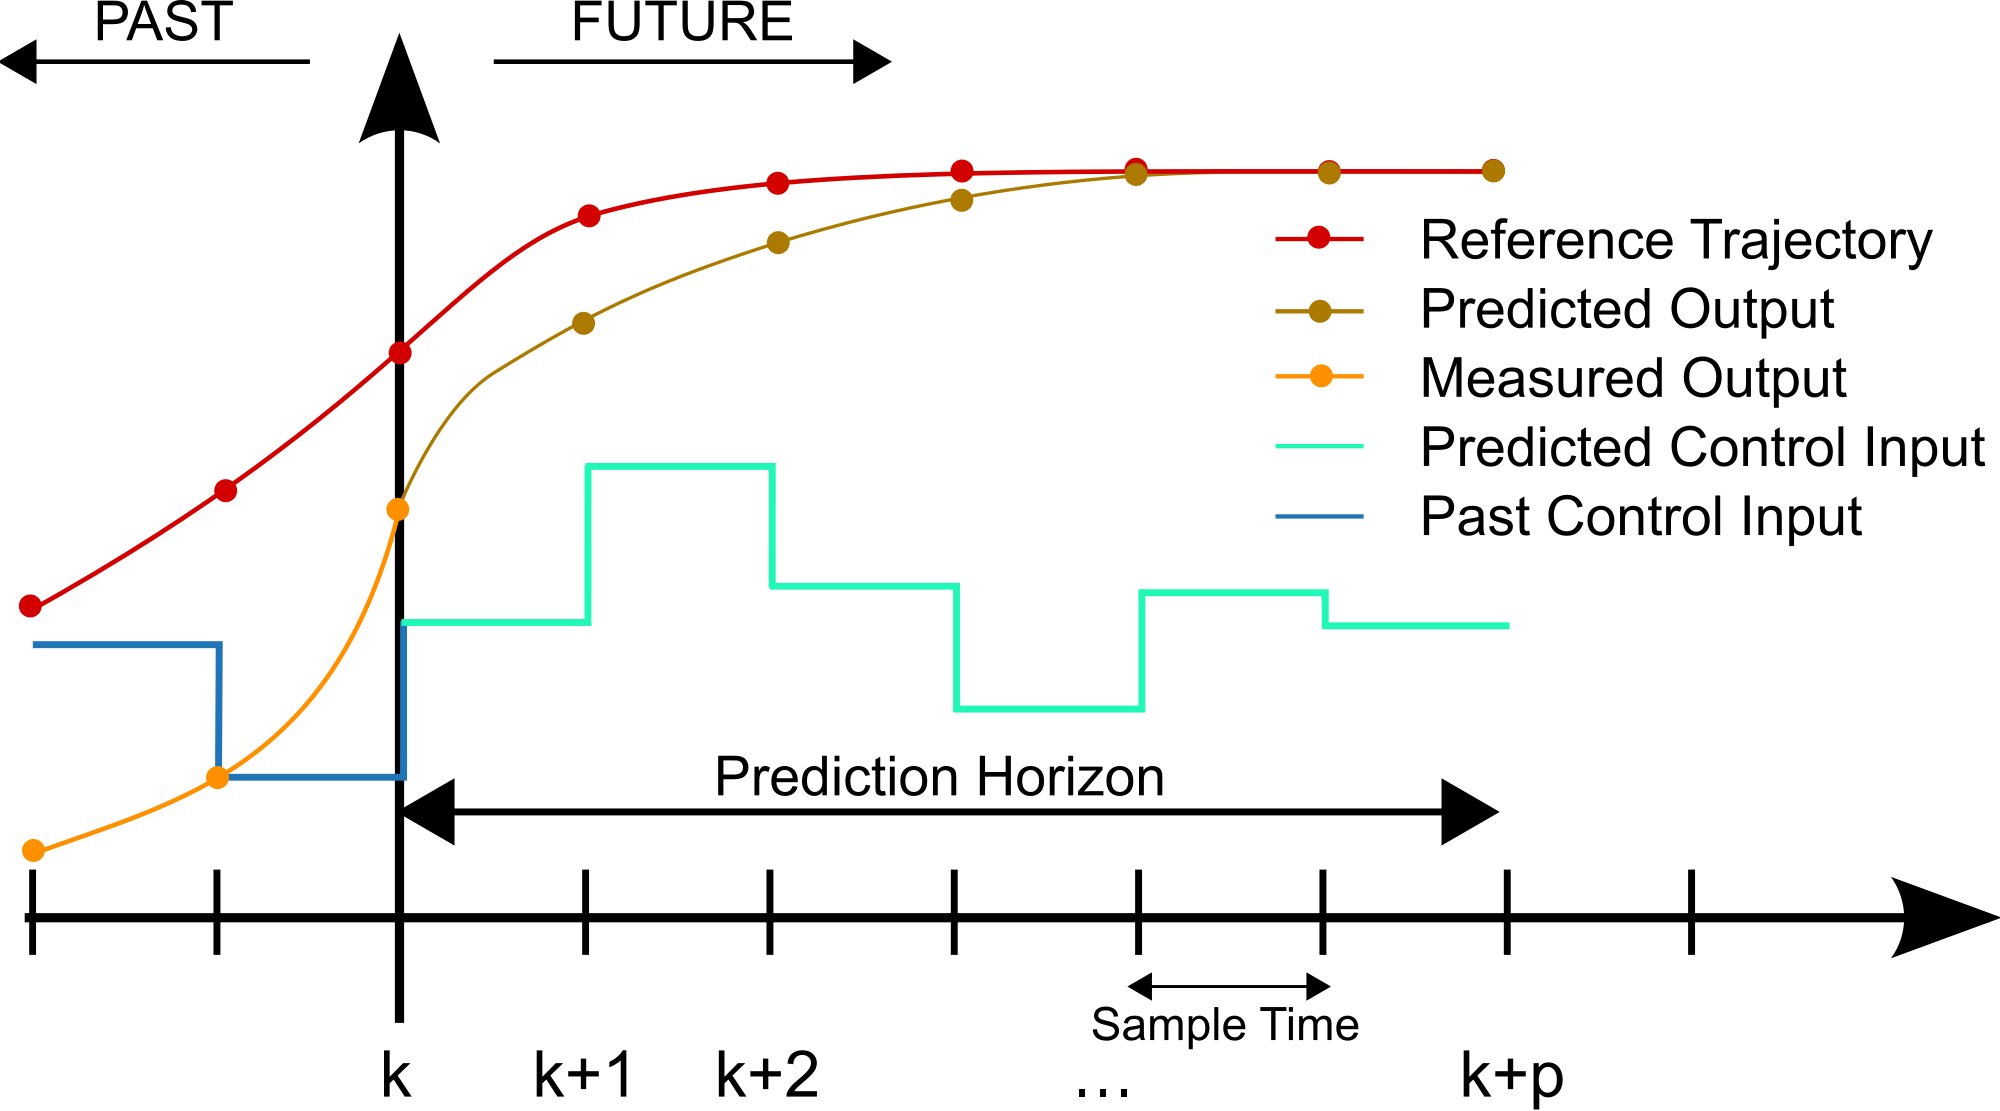
\includegraphics[width=\textwidth]{../figure/mpc_theory.png}
	\caption{A discrete Model Predictive Control scheme adapted from \cite{mpctoolbox}.}
	\label{fig:mpc_theory}
\end{figure}

MPC is typically formulated in the state space. For a given discrete linear time-invariant (LTI) system:
\begin{equation}
\label{eqn:MPC_plant_discrete}
\vec{x}(k+1)=\vec{A}\vec{x}(k)+ \vec{B} \vec{u}(k)
\end{equation}
where $\vec{x}(k)\in\mathbb{R}^n$, $\vec{u}(k)\in\mathbb{R}^m$ are the state and the input, respectively. The central idea in the Model Predictive Control is to minimize some cost function, while still ensuring that some constraints are fulfilled. The generic MPC problem can be written as follows:
\begin{equation}
\label{eqn:MPC_optimization}
\begin{aligned}
& \underset{\textbf{u}}{\text{minimize}}
& & J(\vec{x}(k), \textbf{u}) \\
& \text{subject to}
& & \vec{x}_{k+i+1} = \vec{A}\vec{x}_{k+i}+ \vec{B} \vec{u}_{k+i}\quad\forall i=0,\dots N-1;\\
& & & \vec{x}_{k+i}\in \mathbb{X}\quad\forall i=0,\dots N-1;\\
& & & \vec{u}_{k+i}\in \mathbb{U}\quad\forall i=0,\dots N-1;\\  
& & & \vec{x}_{k+N}\in \mathbb{X}_f;\quad\vec{x}_k = \vec{x}(k).
\end{aligned}
\end{equation}
where $\textbf{u}=(\vec{u}_k,\dots,\vec{u}_{k+N-1})$ is a sequence of control inputs, $\vec{x}_{k+i}$ is the state at time $k+i$ as predicted at time $k$, and $N$ is the prediction horizon. The sets $\mathbb{X}\in\mathbb{R}^n$ and $\mathbb{U}\in\mathbb{R}^m$ define the constraints on the state and the input, respectively. Finally, the set $\mathbb{X}_f\subseteq\mathbb{X}$ defines the terminal constraint on the state. If we consider a regulation problem, the system (\ref{eqn:MPC_plant_discrete}) should be steered to the origin and the cost function $J(\vec{x}(k), \textbf{u})$ could be in a quadratic form as follows:
\begin{equation}
\label{eqn:MPC_cost_function_regulation}
	J(\vec{x}(k), \textbf{u}) = \vec{x}^\intercal_{k+N}\vec{P}_f\vec{x}_{k+N}+\sum_{i=1}^{N}\Big(\vec{x}^\intercal_{k+i}\vec{Q}\vec{x}_{k+i}+\vec{u}_{k+i}^\intercal\vec{R}\vec{u}_{k+i}\Big)
\end{equation}
where $\vec{P}_f,\vec{Q}\geq0$ (positive semi-definite) and $\vec{R}>0$ (positive definite) are weighting matrices.

Instead if we consider a servo problem, like tracking of a reference signal, the cost function is changed as follows:
\begin{equation}
\label{eqn:MPC_cost_function_servo}
\begin{aligned}
J(\vec{x}(k), \textbf{u})=& (\vec{x}_{k+N}-\vec{x}^\text{ref}_{k+N})^\intercal\vec{P}_f(\vec{x}_{k+N}-\vec{x}^\text{ref}_{k+N})\\
&+\sum_{i=1}^{N}\Big((\vec{x}_{k+i}-\vec{x}^\text{ref}_{k+i})^\intercal\vec{Q}(\vec{x}_{k+i}-\vec{x}^\text{ref}_{k+i})+\vec{u}_{k+i}^\intercal\vec{R}\vec{u}_{k+i}\Big)
\end{aligned}
\end{equation}
where $\vec{x}^\text{ref}_{k+i}$, $\vec{x}^\text{ref}_{k+N}$ describe the reference trajectory. The standard MPC algorithm can be summarized by the following steps:
\begin{algorithm}%[b]
	\caption{Basic Model Predictive Control loop}
	\small
	\begin{algorithmic}[1]
		\State Measure the current state $\vec{x}(k)$;
		\State Solve the optimization problem \ref{eqn:MPC_optimization} with $\vec{x}(k)$ as initial state, where $\vec{u}(k)$ is calculated;
		\State Apply the first control of the optimal control sequence;
		\State Wait one sampling time and repeat steps 1-3;
	\end{algorithmic}
	\label{alg:MPCloop}
\end{algorithm}

An MPC has many strengths. Given that the model is discrete and linear it handles multivariable problems very well. Also mathematical convexity is an important part of the resulting problem formulation of an MPC. In fact there exists efficient solvers for convex optimization problems but it is therefore desirable that the MPC problem \ref{eqn:MPC_optimization} is convex which is ensured if:
\begin{enumerate}
\item the cost function is convex;
\item the prediction model is linear;
\item the constraint sets $\mathbb{X}, \mathbb{U}$ are convex.	
\end{enumerate}	
The optimization handles actuator constraints and state constraints naturally in the optimization which allows for
the process to be operated much closer to the hard constraints, which improves control performance and efficiency. Because of its predictive nature it is able to solve a variety of problems and handle disturbances smoothly.

\subsection{Tuning Parameters}
The two most important parameters to tune in order to satisfy the control objectives are the diagonal matrices $\vec{Q}$ and $\vec{R}$ that can be used to weight the system state matrix and the control inputs respectively. The response of the system that is too slow can be influenced by adding high weighting values in the $\vec{Q}$ matrix, whereas the control gains are damped with high weighing values in the $\vec{R}$ matrix. Find an optimal trade-off is a fundamental aspect for the constroller behaviour.

\subsection{Stability of MPC controller}
A limited horizon on the MPC problem affects the stability of the controllers; in order to avoid this problem it is possible to set an infinite horizon, impose end point constraints, terminal cost function or use other techniques. To obtain a stable controller, the parameters to tune are: the terminal cost, prediction horizon and constraints. Also the weights on the cost function can be tuned to ensure a stabilizing solution.

\subsection{Robustness}
If the stability can be guaranteed and the performance specifications are met with respect to a certain set of uncertainties, the system is said to be robust; in particular a controller with this property has to ensure that the constraints are never violated for any admissible disturbance realization. The uncertainties in a system are due to external disturbances, measurement noise, inaccurate values of the model parameters, non-linearities etc...
The most common type of uncertainties considered in the literature is additive disturbance because usually the current state of the system can be measured hence there is no noise in the measurements.

\section{Adaptive Model Predictive Control}
We understood that Model Predictive Control is an advanced method that predicts future behavior using a linear-time-invariant (LTI) dynamic model. These predictions are not exact and a good strategy is to make MPC insensitive to prediction errors. If the plant is strongly nonlinear or its characteristics vary dramatically with time, MPC performance might become unacceptable because LTI prediction accuracy degrade \cite{mpctoolbox}. A method that can address this degradation by adapting the prediction model for changing operating conditions is called Adaptive MPC: this control strategy uses a fixed model structure, but allows the model parameters to evolve with time. Ideally, whenever the controller requires a prediction, it uses a model appropriate for the current conditions. At each control interval, the adaptive MPC controller updates the plant model and nominal conditions. Once updated, the model and conditions remain constant over the prediction horizon. The plant model used as the basis for the adaptive MPC must be an LTI discrete-time, state-space model with a structure as follows:
\begin{equation}
\label{eqn:Adaptive_MPC_plant_discrete}
\begin{aligned}
\vec{x}(k+1)&=\vec{A}\vec{x}(k)+ \vec{B}_u \vec{u}(k)+\vec{B}_v \vec{v}(k)+\vec{B}_d \vec{d}(k)\\
\vec{y}(k)&=\vec{C}\vec{x}(k) + \vec{D}_v \vec{v}(k)+ \vec{D}_d \vec{d}(k)
\end{aligned}
\end{equation}
where the matrices \vec{A}, $\vec{B}_u$, $\vec{B}_v$, $\vec{B}_d$, \vec{C}, $\vec{D}_v$ and $\vec{D}_d$ can vary with time. The other parameters in the previous expression (\ref{eqn:Adaptive_MPC_plant_discrete}) are:
\begin{itemize}
	\item $k$ is the time index/current control interval;
	\item \vec{x} are the plant model states;
	\item \vec{u} are the manipulated inputs that can be adjusted by the MPC controller;
	\item \vec{v} are the measured disturbance inputs;
	\item \vec{d} are the unmeasured disturbance inputs;
	\item \vec{y} are the plant outputs, including both measured (necessary at least one) and unmeasured.
\end{itemize}
In the adaptive MPC control, there are additional requirements for the plant model, like the sample time $T_s$ that has to be constant and identical to the MPC control interval. This control strategy prohibits direct feed-through from any manipulated variable to any plant output. Thus, $\vec{D_v} = \vec{0}$ in the above model.
A traditional MPC controller includes a nominal operating point at which the plant model applies, such as the condition at which you linearize a nonlinear model to obtain the LTI approximation (equilibrium, reference trajectory and the	
most updated value) \cite{mpctoolbox}. In adaptive MPC, as time evolves it should update the nominal operating point to be consistent with the updated plant model. It is possible to rewrite the plant model in terms of deviations from the nominal conditions as follows:
\begin{equation}
\label{eqn:Adaptive_MPC_nominal_condition}
\begin{aligned}
\vec{x}(k+1)&=\overline{\vec{x}}+\vec{A}(\vec{x}(k)-\overline{\vec{x}})+ \vec{B}(\vec{u}_t(k)-\overline{\vec{u}}_t)+\overline{\Delta \vec{x}} \\
\vec{y}(k)&=\overline{\vec{y}}+\vec{C}(\vec{x}(k)-\overline{\vec{x}}) + \vec{D}(\vec{u}_t(k)-\overline{\vec{u}}_t)
\end{aligned}
\end{equation}
where the matrices \vec{A}, \vec{B}, \vec{C} and \vec{D} are updated with respect to time. The other parameters in the previous structure (\ref{eqn:Adaptive_MPC_nominal_condition}) are:
\begin{itemize}
	\item $\vec{u}_t$ is the combined plant input variable, comprising $\vec{u}$, $\vec{v}$ and $\vec{d}$ variables defined earlier;
	\item $\overline{\vec{x}}$ are the nominal states;
	\item $\overline{\Delta \vec{x}}$ are the nominal state increments;
	\item $\overline{\vec{u}_t}$ and $\overline{\vec{y}}$ are the nominal inputs and outputs.
\end{itemize} 
The adaptive MPC uses a Kalman filter to update its controller states which include the plant, the disturbance and measurement noise model states. In particular this filter is linear-time-varying (LTV) because adjusts the gains at each control
interval to maintain consistency with the updated plant model.